\documentclass[11pt,a4paper]{article}

\usepackage[utf8]{inputenc}
\usepackage{parcolumns}
\usepackage{fullpage}
\usepackage[none]{hyphenat}
\usepackage{alltt}
\usepackage{graphicx}
\usepackage{transparent}
\usepackage{eso-pic}

\newcommand\BackgroundPic{%
  \put(0,0){%
    \parbox[b][\paperheight]{\paperwidth}{%
      %% \vfill
      \centering
      {\transparent{0.3}\includegraphics[width=\paperwidth,height=\paperheight,%
        keepaspectratio,page=2,clip = true, trim = 2cm 4cm 0in 0in]{20150406235752619.pdf}}%
      \vfill
            {\transparent{0.3}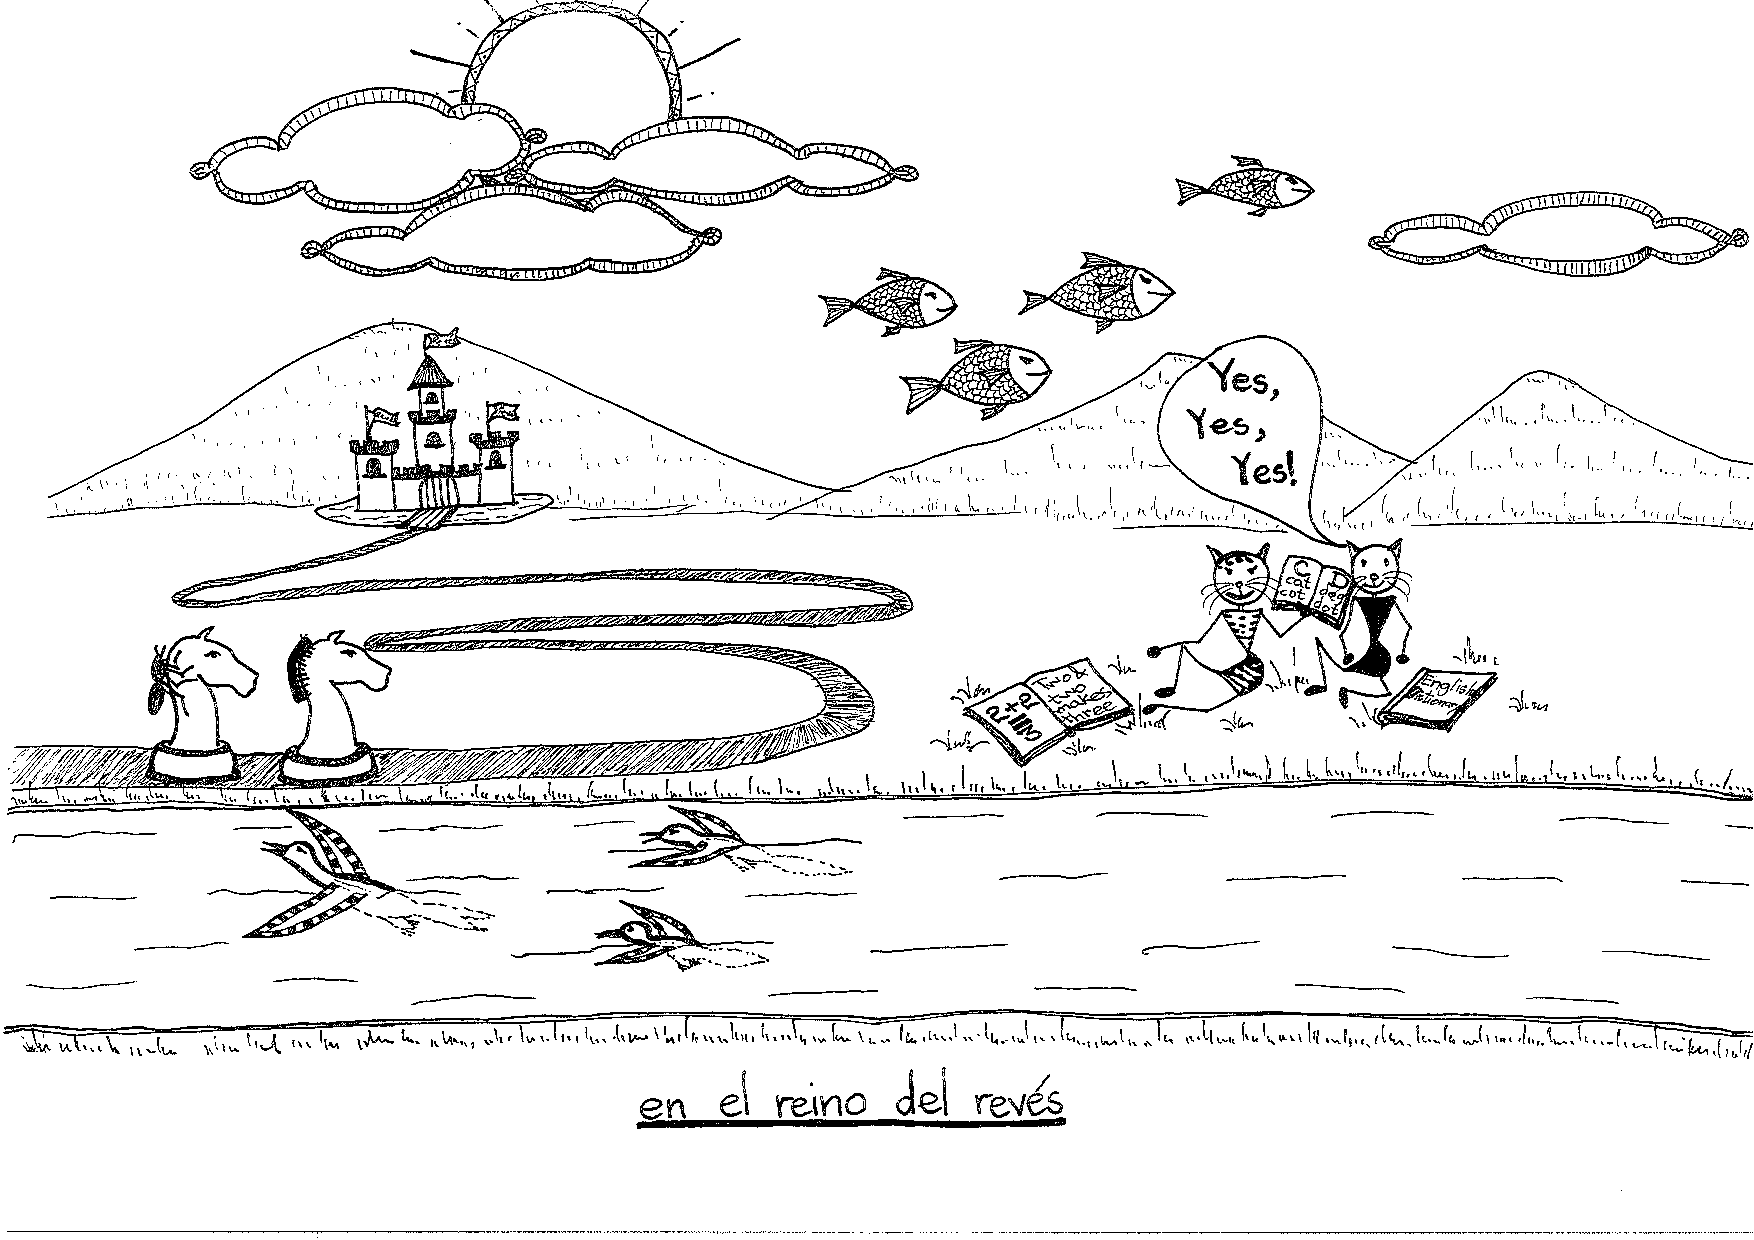
\includegraphics[width=\paperwidth,height=\paperheight,%
        keepaspectratio,page=1,clip = true, trim = 2cm 4cm 0in 0in]{20150406235752619.pdf}}%
      }}}

\date{April 10, 2015}

\begin{document}

\AddToShipoutPicture*{\BackgroundPic}

\phantom{a}
%% \maketitle
\vspace*{\fill}
{\LARGE\textbf{
  \begin{center}
Seis canciones de María Elena Walsh\\
Six Songs of María Elena Walsh
\end{center}
}}
\vspace*{\fill}

\pagestyle{empty}

\clearpage

\setcounter{page}{1}

%% \begin{center}
%% \large
%% \textbf{
%% I\\
%% El Reino del Revés\\
%% The Kingdom of Reverse
%% }
%% \end{center}

\bigskip
\centerline{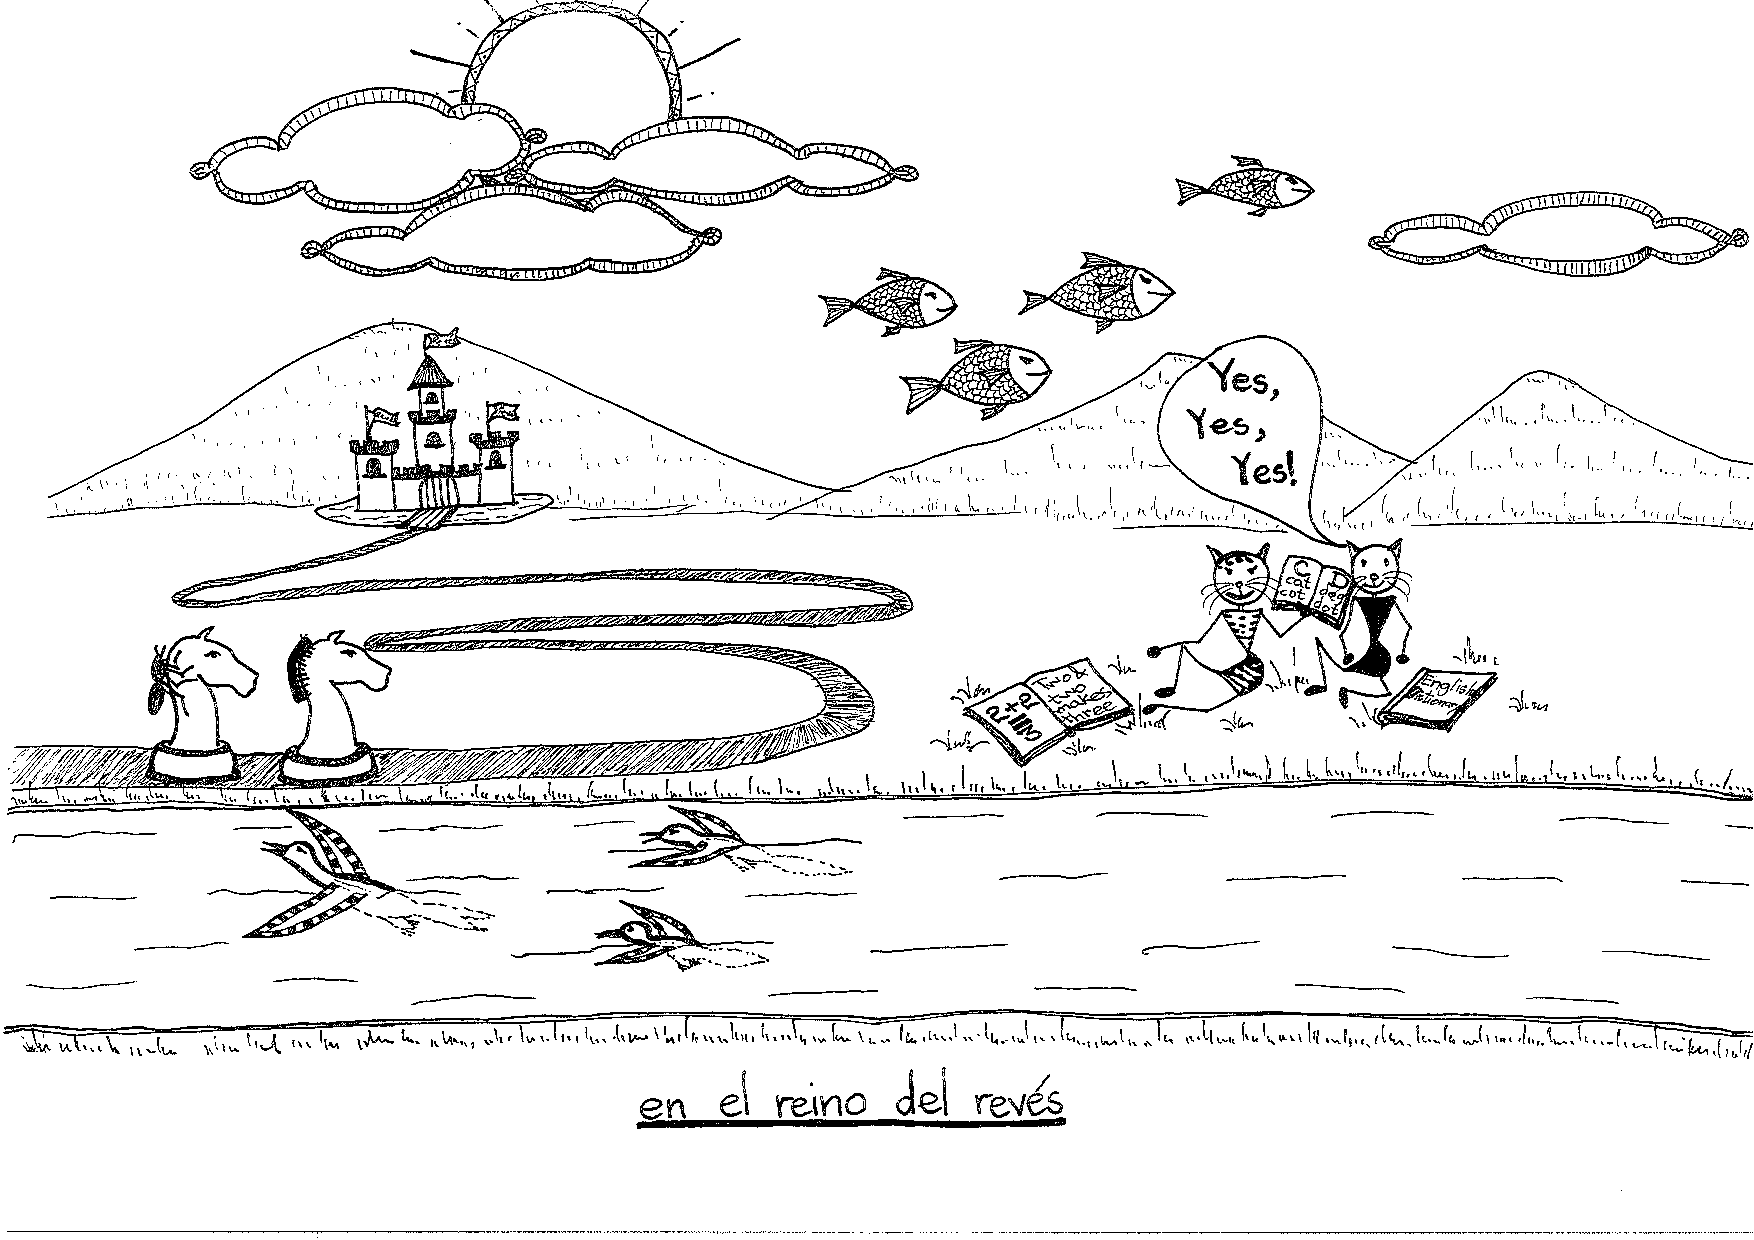
\includegraphics[scale=0.7,clip=true,trim = 0in 3mm 0in 0in]{20150406235752619.pdf}}
\begin{center}\large\textbf{The Kingdom of Reverse}\end{center}

\begin{parcolumns}[distance=8em,nofirstindent=true]{2}

\colchunk
{
\begin{alltt}\normalfont
They told me that in the Kingdom of Reverse
The bird swims and the fish flies,
That the cats don’t say “miau” and that
they say “yes,”
Because they study a lot of English!
\end{alltt}
}

\colchunk{
\begin{alltt}\normalfont
Me dijeron que en el Reino del Revés
nada el pajaro y vuela el pez,
que los gatos no hacen miau y dicen yes
porque estudian mucho ingles!
\end{alltt}
}

\colplacechunks

\colchunk
{
\begin{alltt}\normalfont
We’ll see how it is, the Kingdom of Reverse.
We’ll see how it is, the Kingdom of Reverse!
\end{alltt}
}

\colchunk
{
\begin{alltt}\normalfont
Vamos a ver cómo es, el Reino del Revés\\
Vamos a ver cómo es, el Reino del Revés.
\end{alltt}
}

\colplacechunks

\colchunk
{
\begin{alltt}\normalfont
They told me that in the Kingdom of Reverse
Nobody dances upon their feet,
That one thief is a policeman and another is
a judge,
And that two and two make three!
\end{alltt}
}

\colchunk
{
\begin{alltt}\normalfont
Me dijeron que en el Reino del Revés
nadie baila con los pies,
que un ladrón es vigilante y otro es juez
y que dos y dos son tres.
\end{alltt}
}

\colplacechunks

\colchunk
{
\begin{alltt}\normalfont
We’ll see how it is, the Kingdom of Reverse.
We’ll see how it is, the Kingdom of Reverse!
\end{alltt}
}

\colchunk
{
\begin{alltt}\normalfont
Vamos a ver cómo es, el Reino del Revés
Vamos a ver cómo es, el Reino del Revés.
\end{alltt}
}

\colplacechunks

\colchunk
{
\begin{alltt}\normalfont
They told me that in the Kingdom of Reverse
A bear fits inside a walnut,
That babies have beards and moustaches,
And that a year lasts one month!
\end{alltt}
}

\colchunk
{
\begin{alltt}\normalfont
Me dijeron que en el Reino del Revés
cabe un oso en una nuez,
que usan barbas y bigotes los bebés
y que un año dura un mes.
\end{alltt}
}

\colplacechunks

\colchunk
{
\begin{alltt}\normalfont
We’ll see how it is, the Kingdom of Reverse.
We’ll see how it is, the Kingdom of Reverse!
\end{alltt}
}

\colchunk
{
\begin{alltt}\normalfont
Vamos a ver cómo es, el Reino del Revés
Vamos a ver cómo es, el Reino del Revés.
\end{alltt}
}

\colplacechunks

\colchunk
{
\begin{alltt}\normalfont
They told me that in the Kingdom of Reverse
There is a little dog – a Pekingese,
Who falls upwards, and once
Could not fall back down after!
\end{alltt}
}

\colchunk
{
\begin{alltt}\normalfont
Me dijeron que en el Reino del Revés
hay un perro pekinés
que se cae para arriba y una vez
no pudo bajar después.
\end{alltt}
}

\colplacechunks

\colchunk
{
\begin{alltt}\normalfont
We’ll see how it is, the Kingdom of Reverse.
We’ll see how it is, the Kingdom of Reverse!
\end{alltt}
}

\colchunk
{
\begin{alltt}\normalfont
Vamos a ver cómo es, el Reino del Revés
Vamos a ver cómo es, el Reino del Revés.
\end{alltt}
}

\colplacechunks

\colchunk
{
\begin{alltt}\normalfont
They told me that in the Kingdom of Reverse
A man named Andrés
Has one thousand five hundred and thirty
chimpanzees –
If you look at them, you don’t see them!
\end{alltt}
}

\colchunk
{
\begin{alltt}\normalfont
Me dijeron que en el Reino del Revés
un señor llamado Andrés
tiene 1530 chimpancés
que si miras no los ves.
\end{alltt}
}

\colplacechunks

\colchunk
{
\begin{alltt}\normalfont
We’ll see how it is, the Kingdom of Reverse.
We’ll see how it is, the Kingdom of Reverse!
\end{alltt}
}

\colchunk
{
\begin{alltt}\normalfont
Vamos a ver cómo es, el Reino del Revés
Vamos a ver cómo es, el Reino del Revés.
\end{alltt}
}

\colplacechunks

\colchunk
{
\begin{alltt}\normalfont
They told me that in the Kingdom of Reverse
A spider and a centipede
Go to the palace of the Marquis, mounted
On horses from a game of chess!
\end{alltt}
}

\colchunk
{
\begin{alltt}\normalfont
Me dijeron que en el Reino del Revés
una araña y un ciempies
van montados al palacio del marqués
en caballos de ajedrez.
\end{alltt}
}

\colplacechunks

\colchunk
{
\begin{alltt}\normalfont
We’ll see how it is, the Kingdom of Reverse.
We’ll see how it is, the Kingdom of Reverse!
\end{alltt}
}

\colchunk
{
\begin{alltt}\normalfont
Vamos a ver cómo es, el Reino del Revés
Vamos a ver cómo es, el Reino del Revés.
\end{alltt}
}

\colplacechunks

\end{parcolumns}

\clearpage

%% \begin{center}
%% \large\textbf{
%% II\\
%% La vaca estudiosa\\
%% The Studious Cow
%% }
%% \end{center}

\bigskip
\centerline{\includegraphics[page=2,scale=0.7,clip=true,trim = 0in 3mm 0in 0in]{20150406235752619.pdf}}
\begin{center}\large\textbf{The Studious Cow}\end{center}

\begin{parcolumns}{2}

\colchunk
{
\begin{alltt}\normalfont
There once was a cow
In the ravine of Humahuaca (Oo-ma-oo-aka)
As she was very old, very old,
She was deaf in one ear.
\end{alltt}
}

\colchunk
{
\begin{alltt}\normalfont
Había una vez una vaca
en la quebrada de Humahuaca
Como era muy vieja, muy vieja
estaba sorda de una oreja
\end{alltt}
}

\colplacechunks

\colchunk
{
\begin{alltt}\normalfont
And although she was already a grandmother,
One day, she wanted to go to school.
She put on some red shoes,
Gloves of fine silk, and a pair of spectacles.
\end{alltt}
}

\colchunk
{
\begin{alltt}\normalfont
Y a pesar de que ya era abuela
un día quiso ir a la escuela
Se puso unos zapatos rojos
guantes de tul y un par de anteojos
\end{alltt}
}

\colplacechunks

\colchunk
{
\begin{alltt}\normalfont
The teacher looked at her, terrified,
And said, “You are mistaken!”
And the cow replied to her,
“Why can’t I study?”
\end{alltt}
}

\colchunk
{
\begin{alltt}\normalfont
La vio la maestra asustada
y dijo: "Estás equivocada"
Y la vaca le respondió:
"¿Por qué no puedo estudiar yo?"
\end{alltt}
}

\colplacechunks

\colchunk
{
\begin{alltt}\normalfont
The cow dressed in white
Sat on the first bench.
We children threw chalk
And we died of laughter!
\end{alltt}
}

\colchunk
{
\begin{alltt}\normalfont
La vaca vestida de blanco
se acomodó en el primer banco
Los chicos tirábamos tiza
y nos moríamos de risa
\end{alltt}
}

\colplacechunks

\colchunk
{
\begin{alltt}\normalfont
The people were very curious
To see the studious cow.
People came in trucks,
On bicycles, and in airplanes!
\end{alltt}
}

\colchunk
{
\begin{alltt}\normalfont
La gente se fue muy curiosa
a ver a la vaca estudiosa
La gente llegaba en camiones
en bicicletas y en aviones
\end{alltt}
}

\colplacechunks

\colchunk
{
\begin{alltt}\normalfont
And as the chaos increased
In the school, nobody studied.
The cow, standing in a corner
Ruminated on the lesson alone.
\end{alltt}
}

\colchunk
{
\begin{alltt}\normalfont
Y como el bochinche aumentaba
en la escuela nadie estudiaba
La vaca de pie en un rincón
rumiaba sola la lección
\end{alltt}
}

\colplacechunks

\colchunk
{
\begin{alltt}\normalfont
One day, all of us children,
We became donkeys.
And in that place of Humahuaca
The only wise one was the cow.
\end{alltt}
}

\colchunk
{
\begin{alltt}\normalfont
Un día toditos los chicos
nos convertimos en borricos
Y en ese lugar de Humahuaca
la única sabia fue la vaca
\end{alltt}
}

\colplacechunks

\colchunk
{
\begin{alltt}\normalfont
And in that place of Humahuaca
The only wise one was the cow…
\end{alltt}
}

\colchunk
{
\begin{alltt}\normalfont
Y en ese lugar de Humahuaca
la única sabia fue la vaca...
\end{alltt}
}

\colplacechunks

\end{parcolumns}

\clearpage

%% \begin{center}
%% \large\textbf{
%% III\\
%% Canción de la vacuna \emph{o} El brujito de Gulubú\\
%% The Vaccine Song \emph{or} The Little Wizard of Gulubú
%% }
%% \end{center}

\bigskip
\centerline{\includegraphics[page=3,scale=0.8,clip=true,trim = 4cm 3mm 0in 0in]{20150406235752619.pdf}}
\begin{center}\large\textbf{The Little Wizard of Gulub\'u}\end{center}

\begin{parcolumns}{2}

\colchunk
{
\begin{alltt}\normalfont
There once was a wizard – a little wizard
in Gulubú.
He bewitched the entire population
Without rhyme or reason.
\end{alltt}
}

\colchunk
{
\begin{alltt}\normalfont
Había una vez un bru, un brujito en Gulubú
A toda la población
Embrujaba sin ton ni son
\end{alltt}
}

\colplacechunks

\colchunk
{
\begin{alltt}\normalfont
But one day there came a doctor,
Driving a four-engine truck.
And do you know what happened?
Do you know what happened?
No?
\end{alltt}
}

\colchunk
{
\begin{alltt}\normalfont
Pero un día llegó el doctor
Manejando un cuatrimotor
¿Y saben lo que pasó?
¿Saben lo que pasó?
¿No?
\end{alltt}
}

\colplacechunks

\colchunk
{
\begin{alltt}\normalfont
All the bewitchments
By the little wizard of Gulubú
Were cured with a vac-
With a vaccine!
\end{alltt}
}

\colchunk
{
\begin{alltt}\normalfont
Todas las brujerías
Del brujito de Gulubú
Se curaron con la vacú-
Con la vacuna luna luna lú
\end{alltt}
}

\colplacechunks

\colchunk
{
\begin{alltt}\normalfont
The cow of Gulubú
Could not even say ‘Moo’ –
The little wizard had bewitched her,
And the cow had become mute!
\end{alltt}
}

\colchunk
{
\begin{alltt}\normalfont
La vaca de Gulubú
No podía decir ni mú
El brujito la embrujó
Y la vaca se enmudeció
\end{alltt}
}

\colplacechunks

\colchunk
{
\begin{alltt}\normalfont
But then there came the doctor,
Driving a four-engine truck.
And do you know what happened?
Do you know what happened?
No?
\end{alltt}
}

\colchunk
{
\begin{alltt}\normalfont
Pero entonces llegó el doctor
Manejando un cuatrimotor
¿Y saben lo que pasó?
¿Saben lo que pasó?
¿No?
\end{alltt}
}

\colplacechunks

\colchunk
{
\begin{alltt}\normalfont
All the bewitchments
By the little wizard of Gulubú
Were cured with a vac-
With a vaccine!
\end{alltt}
}

\colchunk
{
\begin{alltt}\normalfont
Todas las brujerías
Del brujito de Gulubú
Se curaron con la vacú-
Con la vacuna luna luna lú
\end{alltt}
}

\colplacechunks

\colchunk
{
\begin{alltt}\normalfont
The children were rather stu-
Stupid in Gulubú.
They forgot the lesson,
Or suffered from measles.
\end{alltt}
}

\colchunk
{
\begin{alltt}\normalfont
Los chicos eran todos muy bu-
Burros todos en Gulubú
Se olvidaban la lección
O sufrían de sarampión
\end{alltt}
}

\colplacechunks

\colchunk
{
\begin{alltt}\normalfont
But one day the doctor arrived,
Driving a four-engine truck.
And do you know what happened?
Do you know what happened?
No?
\end{alltt}
}

\colchunk
{
\begin{alltt}\normalfont
Pero un día llegó el doctor
Manejando un cuatrimotor
¿Y saben lo que pasó?
¿Saben lo que pasó?
¿No?
\end{alltt}
}

\colplacechunks

\colchunk
{
\begin{alltt}\normalfont
All the bewitchments
By the little wizard of Gulubú
Were cured with a vac-
With a vaccine!
\end{alltt}
}

\colchunk
{
\begin{alltt}\normalfont
Todas las brujerías
Del brujito de Gulubú
Se curaron con la vacú-
Con la vacuna luna luna lú
\end{alltt}
}

\colplacechunks

\colchunk
{
\begin{alltt}\normalfont
The little wizard was the one,
The only one in Gulubú
Who wept, kicked and bit
When the doctor pricked him.
\end{alltt}
}

\colchunk
{
\begin{alltt}\normalfont
Ha sido el brujito el ú-
Uno y único en Gulubú
Que lloró, pateó y mordió
Cuando el médico lo pinchó
\end{alltt}
}

\colplacechunks

\colchunk
{
\begin{alltt}\normalfont
And then the doctor marched away,
Driving a four-engine truck
And do you know what happened?
Do you know what happened?
No?
\end{alltt}
}

\colchunk
{
\begin{alltt}\normalfont
Y después se marchó el doctor
Manejando un cuatrimotor
¿Y saben lo que pasó?
¿Saben lo que pasó?
¿No?
\end{alltt}
}

\colplacechunks

\colchunk
{
\begin{alltt}\normalfont
All the bewitchments
By the little wizard of Gulubú
Were cured with a vac-
With a vaccine!
\end{alltt}
}

\colchunk
{
\begin{alltt}\normalfont
Todas las brujerías
Del brujito de Gulubú
Se curaron con la vacú-
Con la vacuna
Luna luna
Lú.
\end{alltt}
}

\colplacechunks

\end{parcolumns}

\clearpage

%% \begin{center}
%% \large\textbf{
%% IV\\
%% La reina batata\\
%% The Sweet Potato Queen
%% }
%% \end{center}

\bigskip
\centerline{\includegraphics[page=4,scale=0.7,clip=true,trim = 0cm 3mm 0cm 0cm]{20150406235752619.pdf}}
\begin{center}\large\textbf{The Sweet Potato Queen}\end{center}

\begin{parcolumns}{2}

\colchunk
{
\begin{alltt}\normalfont
There was the Sweet Potato Queen,
Seated on a platter of silver.
The cook looked at her
And the Queen became bashful.
\end{alltt}
}

\colchunk
{
\begin{alltt}\normalfont
Estaba la reina batata
sentada en un plato de plata
el cocinero la miró
y la reina se abatató.
\end{alltt}
}

\colplacechunks

\colchunk
{
\begin{alltt}\normalfont
The Queen trembled with fear,
And the cook with his finger –
‘No’ and ‘Yes’ and ‘Yes’ and ‘No’ –
In a bad temper, threatened her.
\end{alltt}
}

\colchunk
{
\begin{alltt}\normalfont
La reina temblaba de miedo
y el cocinero con el dedo
que no que si que si que no!
de mal humor la amenazó.
\end{alltt}
}

\colplacechunks

\colchunk
{
\begin{alltt}\normalfont
The Sweet Potato Queen thought,
‘Now he will prick me and kill me.’
The cook murmured,
‘This one, yes, I keep.’
\end{alltt}
}

\colchunk
{
\begin{alltt}\normalfont
Pensaba la reina batata,
ahora me pincha y me mata.
El cocinero murmuró
con esta sí me quedo yo.
\end{alltt}
}

\colplacechunks

\colchunk
{
\begin{alltt}\normalfont
The Queen saw out of the corner of her eye,
That he was sharpening his knife,
And got so, so frightened,
That she rolled to the ground and hid.
\end{alltt}
}

\colchunk
{
\begin{alltt}\normalfont
La reina vió por el rabillo
que estaba afilando el cuchillo
y tanto, tanto se asustó
que rodó al suelo y se escondió.
\end{alltt}
}

\colplacechunks

\colchunk
{
\begin{alltt}\normalfont
Then there arrived from the park
The youngest girl of the house.
When she looked for her yo-yo,
She found her in a corner.
\end{alltt}
}

\colchunk
{
\begin{alltt}\normalfont
Entónces llegó de la plaza
la nena menor de la casa,
cuando buscaba su yo-yo
en un rincón la descubrió.
\end{alltt}
}

\colplacechunks

\colchunk
{
\begin{alltt}\normalfont
The girl, on a throne of tin,
Placed the Sweet Potato Queen.
A little tail of green she sprouted –
(The Sweet Potato Queen, not the girl!) –
And with that this song ends.
\end{alltt}
}

\colchunk
{
\begin{alltt}\normalfont
La nena en un trono de lata,
la puso a la reina batata
colita verde le brotó.
(a la reina batata a la nena no)
y esta canción se terminó.
\end{alltt}
}

\colplacechunks

\end{parcolumns}

\clearpage

%% \begin{center}
%% \large\textbf{
%% V\\
%% Canción para vestirse\\
%% Song to Dress Oneself
%% }
%% \end{center}

\bigskip
\centerline{\includegraphics[page=5,scale=0.7,clip=true,trim = 8cm 3mm 4cm 4cm]{20150406235752619.pdf}}
\begin{center}\large\textbf{Song to Dress Oneself}\end{center}

\begin{parcolumns}{2}

\colchunk
{
\begin{alltt}\normalfont
Upon awaking,
Said the frog,
As he espied
From his window:
\end{alltt}
}

\colchunk
{
\begin{alltt}\normalfont
A levantarse,
dijo la rana,
mientras espiaba
por la ventana.
\end{alltt}
}

\colplacechunks

\colchunk
{
\begin{alltt}\normalfont
‘\emph{Lace with a little lace,
And a buttonhole with a button.}’
\end{alltt}
}

\colchunk
{
\begin{alltt}\normalfont
\emph{Tira con tirita
y ojal con botón.}
\end{alltt}
}

\colplacechunks

\colchunk
{
\begin{alltt}\normalfont
A little bird
That was in bed
Searches for its shoe
Beneath the branch.
\end{alltt}
}

\colchunk
{
\begin{alltt}\normalfont
Un pajarito
que está en la cama
busca el zapato
bajo la rama.
\end{alltt}
}

\colplacechunks

\colchunk
{
\begin{alltt}\normalfont
\emph{Lace with a little lace,
And a buttonhole with a button.}
\end{alltt}
}

\colchunk
{
\begin{alltt}\normalfont
\emph{Tira con tirita
y ojal con botón.}
\end{alltt}
}

\colplacechunks

\colchunk
{
\begin{alltt}\normalfont
‘Upa,’ said
Four mice,
And they took off
Their nightshirts.
\end{alltt}
}

\colchunk
{
\begin{alltt}\normalfont
Aupa, dijeron
cuatro ratones,
y se quitaron
los camisones.
\end{alltt}
}

\colplacechunks

\colchunk
{
\begin{alltt}\normalfont
\emph{Lace with a little lace,
And a buttonhole with a button.}
\end{alltt}
}

\colchunk
{
\begin{alltt}\normalfont
\emph{Tira con tirita
y ojal con botón.}
\end{alltt}
}

\colplacechunks

\colchunk
{
\begin{alltt}\normalfont
‘I can’t find my flute,’
Complained the cricket,
And he had it
In his pocket.
\end{alltt}
}

\colchunk
{
\begin{alltt}\normalfont
No hallo mi flauta,
protestó el grillo,
y la tenía
en el bolsillo.
\end{alltt}
}

\colplacechunks

\colchunk
{
\begin{alltt}\normalfont
\emph{Lace with a little lace,
And a buttonhole with a button.}
\end{alltt}
}

\colchunk
{
\begin{alltt}\normalfont
\emph{Tira con tirita
y ojal con botón.}
\end{alltt}
}

\colplacechunks

\colchunk
{
\begin{alltt}\normalfont
A hen
Dying of laughter
Puts on a cap
And a shirt.
\end{alltt}
}

\colchunk
{
\begin{alltt}\normalfont
Una gallina
muerta de risa
se pone el gorro
y la camisa.
\end{alltt}
}

\colplacechunks

\colchunk
{
\begin{alltt}\normalfont
\emph{Lace with a little lace,
And a buttonhole with a button.}
\end{alltt}
}

\colchunk
{
\begin{alltt}\normalfont
\emph{Tira con tirita
y ojal con botón.}
\end{alltt}
}

\colplacechunks

\colchunk
{
\begin{alltt}\normalfont
Half asleep
Says the cat,
‘When I rise early,
I always grumble.’
\end{alltt}
}

\colchunk
{
\begin{alltt}\normalfont
Medio dormido
dice el morrongo:
"Cuando madrugo
siempre rezongo".
\end{alltt}
}

\colplacechunks

\colchunk
{
\begin{alltt}\normalfont
\emph{Lace with a little lace,
And a buttonhole with a button.}
\end{alltt}
}

\colchunk
{
\begin{alltt}\normalfont
\emph{Tira con tirita
y ojal con botón.}
\end{alltt}
}

\colplacechunks

\colchunk
{
\begin{alltt}\normalfont
And the toad says,
‘What folly
To breakfast
With chocolate!’
\end{alltt}
}

\colchunk
{
\begin{alltt}\normalfont
Y el sapo dice:
"¡Qué disparate,
desayunarse
con chocolate!"
\end{alltt}
}

\colplacechunks

\colchunk
{
\begin{alltt}\normalfont
\emph{Lace with a little lace,
And a buttonhole with a button.}
\end{alltt}
}

\colchunk
{
\begin{alltt}\normalfont
\emph{Tira con tirita
y ojal con botón.}
\end{alltt}
}

\colplacechunks

\colchunk
{
\begin{alltt}\normalfont
\emph{Lace with a little lace,
And a buttonhole with a button.}
\end{alltt}
}

\colchunk
{
\begin{alltt}\normalfont
\emph{Tira con tirita
y ojal con botón.}
\end{alltt}
}

\colplacechunks

\end{parcolumns}

\clearpage

%% \begin{center}
%% \large\textbf{
%% VI\\
%% Canción de tomar el té\\
%% Song of Drinking Tea
%% }
%% \end{center}

\bigskip
\centerline{\includegraphics[page=6,scale=0.7,clip=true,trim = 6.9cm 3mm 0cm 3cm]{20150406235752619.pdf}}
\begin{center}\large\textbf{Song of Drinking Tea}\end{center}

\begin{parcolumns}{2}

\colchunk
{
\begin{alltt}\normalfont
We are invited to drink tea.
The teapot is of porcelain
But one doesn’t see it,
I don’t know why.
\end{alltt}
}

\colchunk
{
\begin{alltt}\normalfont
Estamos invitados a tomar el té.
La tetera es de porcelana
Pero no se ve,
Yo no sé por qué.
\end{alltt}
}

\colplacechunks

\colchunk
{
\begin{alltt}\normalfont
The milk feels cold,
And I would wrap her up
I would put my overcoat on her,
Long until her feet,
I don’t know why.
\end{alltt}
}

\colchunk
{
\begin{alltt}\normalfont
La leche tiene frío
Y la abrigaré,
Le pondré un sobretodo mío
Largo hasta los pies,
Yo no sé por qué.
\end{alltt}
}

\colplacechunks

\colchunk
{
\begin{alltt}\normalfont
Be careful when you drink,
It may fall down.
Your nose inside the cup,
And that is not alright,
I don’t know why.
\end{alltt}
}

\colchunk
{
\begin{alltt}\normalfont
Cuidado cuando beban,
Se les va a caer
La nariz dentro de la taza
Y eso no esta bien,
Yo no sé por qué.
\end{alltt}
}

\colplacechunks

\colchunk
{
\begin{alltt}\normalfont
Behind a piece of toast,
Hid the honey;
The butter, very angry,
Told her off in English,
I don’t know why.
\end{alltt}
}

\colchunk
{
\begin{alltt}\normalfont
Detrás de una tostada
Se escondió la miel,
La manteca muy enojada
La retó en inglés,
Yo no sé por qué.
\end{alltt}
}

\colplacechunks

\colchunk
{
\begin{alltt}\normalfont
Tomorrow they take prisoner
A colonel,
For pricking the marmalade
With a pin.
I don’t know why.
\end{alltt}
}

\colchunk
{
\begin{alltt}\normalfont
Mañana se lo llevan preso
A un coronel
Por pinchar a la mermelada
Con un alfiler,
Yo no sé por qué.
\end{alltt}
}

\colplacechunks

\colchunk
{
\begin{alltt}\normalfont
It seems the sugar
Was always black,
And a fright made her white
As you see her,
I don’t know why.
\end{alltt}
}

\colchunk
{
\begin{alltt}\normalfont
Parece que el azúcar
Siempre negra fue
Y de un susto se puso blanca
Tal como la ven,
Yo no sé por qué.
\end{alltt}
}

\colplacechunks

\colchunk
{
\begin{alltt}\normalfont
A timid plate
Got married the day before yesterday,
To his wife, the coffee pot,
He treats her formally,
I don’t know why.
\end{alltt}
}

\colchunk
{
\begin{alltt}\normalfont
Un plato timorato
Se casó anteayer.
A su esposa la cafetera
La trata de usted,
Yo no sé por qué.
\end{alltt}
}

\colplacechunks

\colchunk
{
\begin{alltt}\normalfont
The poor strainers
Are very thirsty,
Because the water escapes from them,
Every so often,
I don’t know why.
\end{alltt}
}

\colchunk
{
\begin{alltt}\normalfont
Los pobres coladores
Tienen mucha sed
Porque el agua se les escapa
Cada dos por tres,
Yo no sé por qué.
\end{alltt}
}

\colplacechunks

\end{parcolumns}

\end{document}
